\documentclass{article}
\usepackage[left=3cm, right=3cm, top=2cm, bottom=2cm]{geometry}
\usepackage[colorlinks=true, allcolors=blue]{hyperref}
\usepackage{tikz}

\title{Data Structures and Algorithms Spring 2024 — Problem Sets}
\author{by Asqar Arslanov}
\date{\today}

\begin{document}
\maketitle{\section*{Week 13. Problem set}}

\begin{enumerate}
    \item Run the Floyd-Warshall algorithm~\cite[\S 23.2]{cormen} on the following graph. Use the alphabetic
          order of vertices. Show the state of distance matrix \(D\) after each iteration of outer loop in the
          algorithm. Since the graph has \(5\) vertices, you must provide five \(5 \times 5\) matrices in your answer.
          No justification is required.
          
          \begin{center}
              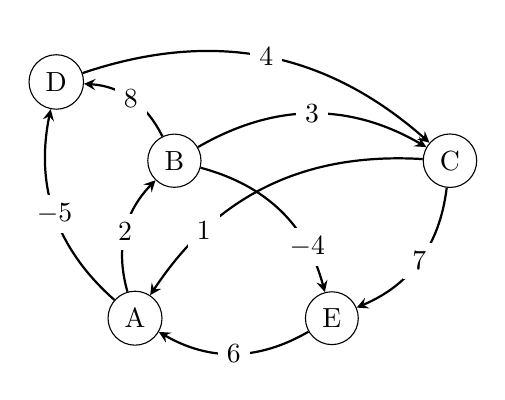
\begin{tikzpicture} [
                      thick,
                      every node/.style={fill=white},
                      vertex/.style={thin, draw, circle},
                  ]
                  \path {
                      (+0.0, +0.0) node [vertex] (A) {A}
                      (+0.5, +2.0) node [vertex] (B) {B}
                      (+4.0, +2.0) node [vertex] (C) {C}
                      (-1.0, +3.0) node [vertex] (D) {D}
                      (+2.5, +0.0) node [vertex] (E) {E}
                  };
                  \draw[-stealth] (A) to [bend left]  node [midway]   {\(2\)}  (B);
                  \draw[-stealth] (A) to [bend left]  node [midway]   {\(-5\)} (D);
                  \draw[-stealth] (B) to [bend left]  node [midway]   {\(3\)}  (C);
                  \draw[-stealth] (B) to [bend right] node [midway]   {\(8\)}  (D);
                  \draw[-stealth] (B) to [bend left]  node [near end] {\(-4\)} (E);
                  \draw[-stealth] (C) to [bend right] node [near end] {\(1\)}  (A);
                  \draw[-stealth] (C) to [bend left]  node [midway]   {\(7\)}  (E);
                  \draw[-stealth] (D) to [bend left]  node [midway]   {\(4\)}  (C);
                  \draw[-stealth] (E) to [bend left]  node [midway]   {\(6\)}  (A);
              \end{tikzpicture}
          \end{center}
          
    \item Provide a graph with exactly \(4\) vertices (A, B, C, D) and \(4\) weighted edges, such that Dijkstra's
          algorithm~\cite[\S 22.3]{cormen} does \textbf{not} give a correct shortest distance for at least one vertex:
          
          \begin{enumerate}
              \item Provide the graph (the graph must be rendered in a clear way, text representation is not
                    enough); Weights must be (small) integers.
                    
              \item Provide the result of Dijkstra's algorithm for each vertex: any shortest path \textbf{and} corre-
                    sponding total weight;
                    
              \item Provide the correct shortest path and corresponding total weight for each vertex;
                    
              \item Explain why Dijkstra's algorithm did not provide the correct answer (specifically for your
                    example, generic justification is not accepted).
          \end{enumerate}
          
    \item Since Dijkstra's shortest paths algorithm~\cite[\S 22.3]{cormen} does not work with negative edges in
          general, consider an algorithm that, for a given graph \(G\), if it has a negative edge, finds the
          minimum edge in \(G\) with the weight \((-W)\) and adds \((+W)\) to all edges in the original graph,
          resulting in a new graph \(G^{+W}\). Then the modified algorithm runs Dijkstra's algorithm on \(G^{+W}\).
          Are the resulting shortest paths in \(G^{+W}\) also shortest in \(G\)? If yes, prove it. If no, provide a
          concrete counterexample and a justification.
\end{enumerate}

\begin{thebibliography}{.week-13.}
    \bibitem[Cormen]{cormen} T. H. Cormen, C. E. Leiserson, R. L. Rivest and C. Stein.\ \emph{Introduction to Algorithms,
        Fourth Edition}. The MIT Press 2022
\end{thebibliography}
\end{document}
